\chapter{Introduction}

Large language models (LLMs) have achieved strong performance on a wide range of language tasks. However, small models (sub-4B parameters) often fall short on multi-step reasoning benchmarks such as GSM8K, where solutions require decomposing a problem into intermediate steps and computing a precise numeric answer \cite{cobbe2021trainingverifierssolvemath}. Chain-of-thought (CoT) prompting can elicit step-by-step reasoning from strong teachers and improve accuracy \cite{wei2023chainofthoughtpromptingelicitsreasoning}, especially when combined with self-consistency sampling \cite{wang2023selfconsistencyimproveschainthought}. Yet, relying on large models at inference time is costly and slow. This motivates distilling teacher reasoning traces into a small student that can run efficiently on commodity hardware.

This thesis studies supervised chain-of-thought distillation (SCoTD): a strong teacher generates structured CoTs for GSM8K questions; a small student is finetuned to reproduce these traces and final answers. The student is trained with parameter-efficient finetuning (LoRA) \cite{hu2021loralowrankadaptationlarge} on quantized weights (QLoRA) \cite{dettmers2023qloraefficientfinetuningquantized}, enabling training on a single 24GB GPU while preserving headroom to learn reasoning behavior. The approach uses standard open-source tooling for models and tokenization \cite{wolf2020huggingfacestransformersstateoftheartnatural,kudo2018sentencepiecesimplelanguageindependent,sennrich2016neuralmachinetranslationrare}.

\section*{Problem and motivation}
Small models are attractive due to their lower latency, footprint, and cost, but they struggle with multi-step math reasoning under greedy decoding. CoT distillation promises to transfer the teacher’s intermediate reasoning patterns, potentially improving student accuracy without increasing inference-time cost. The practical question is whether a 3B-class model can benefit sufficiently from SCoTD to close part of the gap to teacher performance on GSM8K.

\section*{Research questions}
\begin{itemize}
    \item RQ1: Does SCoTD improve a 3B-class model on GSM8K compared to the non-finetuned base under CoT prompting?
    \item RQ2: How does label-only supervised finetuning compare to SCoTD and base baselines under strict numeric exact-match evaluation?
\end{itemize}

\section*{Scope}
The study focuses on a single small decoder-only model (Qwen2.5-3B) \cite{qwen2025qwen25technicalreport} and a single dataset (GSM8K) \cite{cobbe2021trainingverifierssolvemath}. Teacher CoTs are produced via an API-accessible, strong reasoning model configured to emit structured steps and a line-form final answer. The student is trained with LoRA on 4-bit quantized base weights using bf16 compute, gradient checkpointing, and standard optimizers. Evaluation uses greedy decoding with strict numeric parsing; outputs that deviate from the expected format are counted as incorrect.

\section*{Contributions}
\begin{itemize}
    \item A practical, cost-aware pipeline for generating and cleaning teacher CoTs for GSM8K, with concurrency-tuned API calls and per-sample metadata for analysis.
    \item A reproducible PEFT training setup (LoRA + 4-bit nf4 + bf16) that fits on a single 24GB GPU while targeting attention and MLP projection modules.
    \item Empirical evidence that SCoTD improves a 3B-class model over base CoT prompting on GSM8K (78.54\% vs 70.51\%), with a strong teacher at 93.61\% and a label-only student that improves over baseline (15.01\% vs 10.99\%) despite strict-format penalties.
    \item Operational notes on prompt design, cleaning/deduplication, truncation policy, and evaluation pitfalls that affect measured accuracy.
\end{itemize}

\section*{Method overview}
The pipeline comprises teacher CoT generation, cleaning and deduplication, dataset processing, student finetuning (SCoTD and label-only variants), and evaluation. The student relies on PEFT with LoRA adapters \cite{hu2021loralowrankadaptationlarge} over a quantized backbone \cite{dettmers2023qloraefficientfinetuningquantized}. Tokenization is handled with a fast subword tokenizer \cite{kudo2018sentencepiecesimplelanguageindependent,sennrich2016neuralmachinetranslationrare}. Inference uses greedy decoding and a strict numeric exact-match metric. The software stack builds on Transformers and related tooling \cite{wolf2020huggingfacestransformersstateoftheartnatural}. The teacher is a strong reasoning model (DeepSeek-R1 Distill \cite{deepseekai2025deepseekr1incentivizingreasoningcapability}) accessed via OpenRouter \cite{openrouter}.

\begin{figure}[!h]
    \centering
    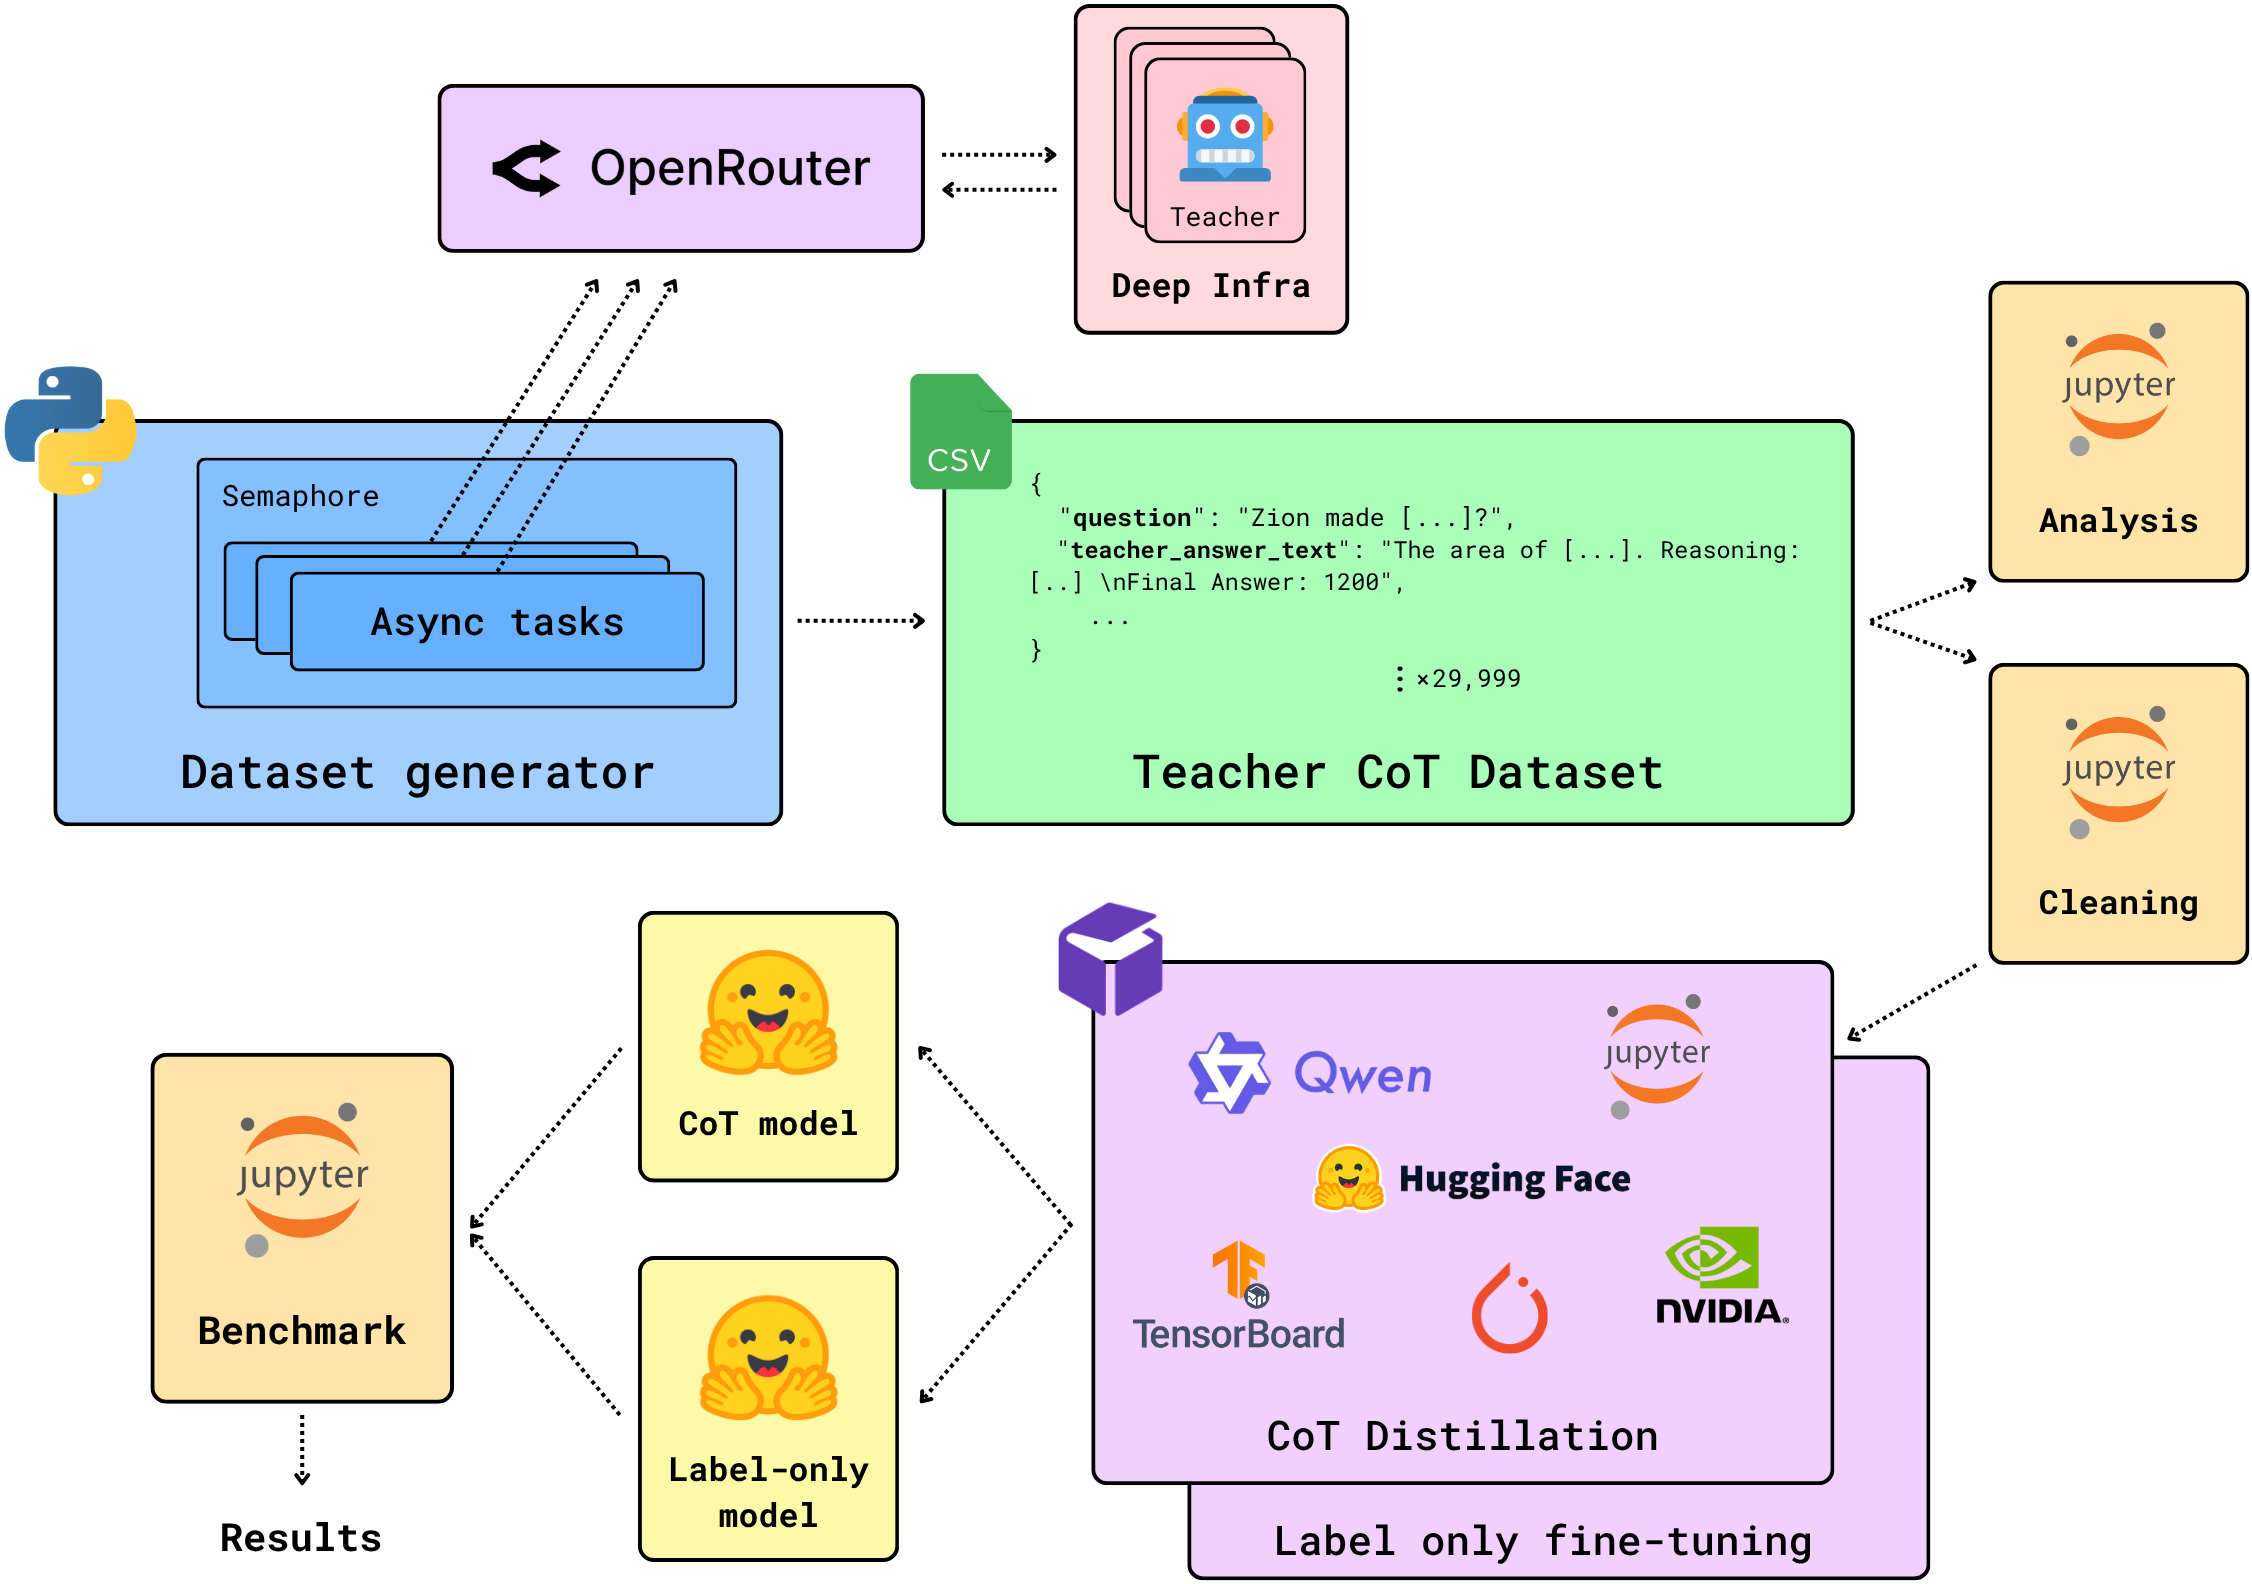
\includegraphics[width=\linewidth]{img/pipeline.png}
    \caption{End-to-end SCoTD pipeline.}
    \label{fig:pipeline-overview}
\end{figure}

\section*{Results summary}
SCoTD yields a clear gain over the base model under CoT prompting (78.54\% vs 70.51\%). Label-only finetuning improves over its baseline (15.01\% vs 10.99\%), though strict formatting likely undercounts correct numeric computations. The teacher achieves 93.61\% on GSM8K test, providing headroom and confirming the value of distilling high-quality reasoning traces.

\section*{Author background and motivation}
The author is a Co-Founder at an AI phishing detection startup that uses LLMs to analyze URLs and webpage content for malicious indicators, and a Machine Learning Engineer at OneRail building LLM-powered support workflows for same-day logistics. These roles highlighted the need for reliable, cost-efficient reasoning under tight latency and single-GPU constraints, motivating SCoTD as a practical path to higher accuracy.